\documentclass[../report.tex]{subfiles}
\begin{document}
	
\section{Manage Data}

In PyTorch, there are conventions to be followed when using datasets. In our case, the dataset consists of images from the \textbf{Caltech101 dataset} (found in \texttt{torchvision.datasets}), specifically the \textbf{airplane dataset}. In the package \href{https://github.com/cMancio00/Super-Resolution/blob/main/dataset/data_preparation.py}{dataset}, there is a module called \texttt{data\_preparation.py}, which contains a function to download this dataset into the \textbf{data} folder of the project.

\subsection{Dataset class}

As mentioned before, in PyTorch, we should use a convention to easily manage datasets. We need to extend the dataset class. The result is a \textbf{SuperResolutionDataset} class found in \href{https://github.com/cMancio00/Super-Resolution/blob/main/dataset/super_resolution_dataset.py}{dataset/super\_resolution\_dataset.py}.

\begin{lstlisting}[style=python, language=python, label={lst:SuperResolutionDataset}, caption={SuperResolutionDataset}]
class SuperResolutionDataset(Dataset):
	def __init__(self, root_dir, transform=transforms.Compose([transforms.ToTensor()])) -> None:
		self.root_dir = root_dir
		self.transform = transform
		self.file_names = os.listdir(root_dir)

	def __len__(self) -> int:
	return len(self.file_names)

	def __getitem__(self, idx) -> tuple[torch.Tensor, torch.Tensor]:
		img_path = os.path.join(self.root_dir, self.file_names[idx])
		image = Image.open(img_path)
		low_res = image.resize((128, 64))
		high_res = image.resize((256, 128))
	
		if self.transform:
		low_res = self.transform(low_res)
		high_res = self.transform(high_res)
		
	return low_res, high_res
\end{lstlisting}
As we can see in listing \ref{lst:SuperResolutionDataset}, we have to define a function to get the length of the dataset and a function to specify what happens during access with an index. In our case, we return two tensors containing the low-resolution and high-resolution representations of the images.
\subsection{Splitting and loading the dataset}
For splitting and loading the dataset we have to use the class that we have implemented.
\begin{lstlisting}[style=python, language=python, label={lst:Splitting}, caption={Splitting}]
def split_dataset(dataset: Dataset, sizes: dict[str, float]) -> list[Subset]:
	required_keys = {'train', 'validation', 'test'}
	if set(required_keys) != set(sizes.keys()):
	raise ValueError(f"Dictionary of sizes must contain 'train', 'validation', and 'test' keys")
	if not sum(sizes.values()) == 1.0:
	raise ValueError(f"Sizes do not summ up to 1.0,but got {sum(sizes.values()):.2f}")
	train_size = int(sizes["train"] * len(dataset))
	validation_size = int(sizes["validation"] * len(dataset))
	test_size = len(dataset) - train_size - validation_size
return torch.utils.data.random_split(dataset, [train_size, validation_size, test_size])
\end{lstlisting}
The splitting function shown in listing \ref{lst:Splitting} takes a dictionary with percentages as input (which must sum to 1) and returns three disjoint datasets that have been randomly split.\\
To load and utilize the dataset, we pass it to the \texttt{DataLoader} class, which is a standard approach in PyTorch. We can also specify the batch size and whether we want to shuffle the dataset when selecting batches.\\
An example of how to use it is provided in listing \ref{lst:DataLoader}.
\begin{lstlisting}[style=python, language=python, label={lst:DataLoader}, caption={Example of DataLoader}]
download("./data", "airplanes")
root_dir = 'data/airplanes'
dataset = SuperResolutionDataset(root_dir=root_dir)
dataset_dataloader = DataLoader(dataset, batch_size=16, shuffle=True)
\end{lstlisting}
Iterating through the DataLoader we can get a similar output as shown in Fig. \ref{fig:example_of_output}.
\begin{figure}[H]
	\caption{Example Output of DataLoader}
	\centering
	\label{fig:example_of_output}
	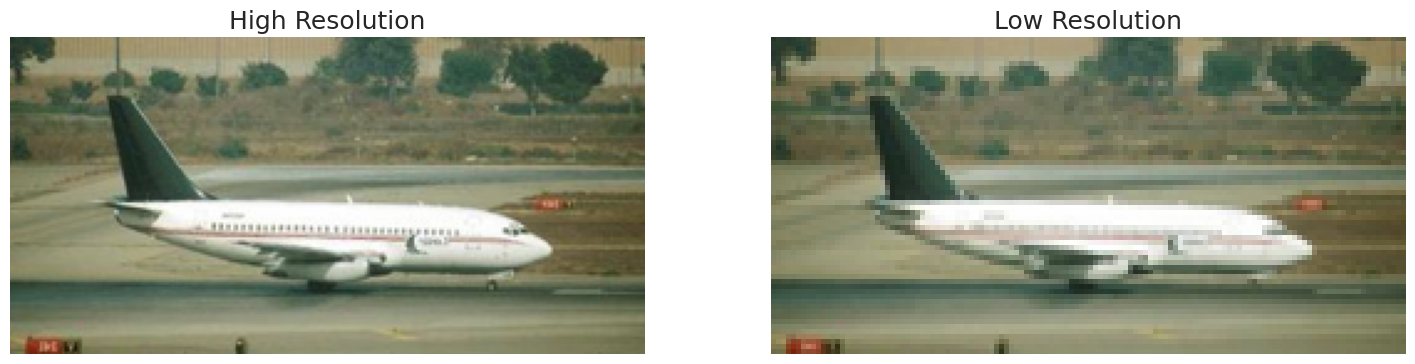
\includegraphics[width=\textwidth]{../images/Example_of_Output.png}
\end{figure}
\end{document}
